%%%%%%%%%%%%%%%%%%%%
%%%%%%%%%%%%%%%%%%%%

\begin{frame}
%    \shiftedframetitle{2. Theory}
%\begin{itemize}
%\item NS discussion
%\item SWE derivation
%\end{itemize}
    \shiftedframetitle{2. Theory - {\large Shallow Water Equations  model {\small  (initial)}}}

%\vspace{-3mm}
\begin{minipage}{0.35\textwidth}
\begin{itemize}
\item<1->[]
\begin{align*}
\frac{\partial u}{\partial x} + \frac{\partial v}{\partial y} + \frac{\partial w}{\partial z} &= 0
\end{align*}
\item<1->[]
\begin{align*}
\frac{\partial u}{\partial t} + u\frac{\partial u}{\partial x} + v\frac{\partial u}{\partial y} + w\frac{\partial u}{\partial z} &= - \frac{\partial p}{\partial x}
\end{align*}
\item<1->[]
\begin{align*}
\frac{\partial v}{\partial t} + u\frac{\partial v}{\partial x} + v\frac{\partial v}{\partial y} + w\frac{\partial v}{\partial z}&= - \frac{\partial p}{\partial y}
\end{align*}
\item<1->[]
\begin{align*}
\frac{\partial w}{\partial t} + u\frac{\partial w}{\partial x} + v\frac{\partial w}{\partial y} + w\frac{\partial w}{\partial z} &= - \frac{\partial p}{\partial z} + g \end{align*}
\end{itemize}
\end{minipage}
\hspace{1.5cm}
\begin{minipage}{0.35\textwidth}
\includegraphics[scale=0.65]{./Resources/Images/imagesThesis/floor.png}%
\end{minipage}
\end{frame}
\clearpage

%%%%%%%%%%%%%%%%%%%%
%%%%%%%%%%%%%%%%%%%%

\begin{frame}
    \shiftedframetitle{2. Theory - {\large Shallow Water Equations  model {\small  (initial)}}}
\vspace{-0.5cm}
\begin{minipage}{0.3\textwidth}
\begin{itemize}
\item<1->[]
\begin{align*}
\color{TUMOrange}\underbrace{\color{black}\frac{\partial u}{\partial x} + \frac{\partial v}{\partial y}}_{\approx \frac{2U}{L}} \color{black} + \color{TUMOrange}\underbrace{\color{black}\frac{\partial w}{\partial z}}_{\myTUMorange{\approx \frac{W}{H}}} &= 0 \quad \myTUMorange{\rightarrow} \quad \color{TUMOrange}\underbrace{W \approx -2U \frac{H}{L}}_{\approx\ 0 \ if\  L>>H} \qquad \qquad \quad
\end{align*}
\item<2->[]
\begin{align*}
\frac{\partial u}{\partial t} + u\frac{\partial u}{\partial x} + v\frac{\partial u}{\partial y} + w\frac{\partial u}{\partial z} &= - \frac{\partial p}{\partial x}\\[0.5cm]
\frac{\partial v}{\partial t} + u\frac{\partial v}{\partial x} + v\frac{\partial v}{\partial y} + w\frac{\partial v}{\partial z}&= - \frac{\partial p}{\partial y}\\[0.5cm]
\color{TUMDarkBlue}\underbrace{\color{black}\frac{\partial w}{\partial t} + u\frac{\partial w}{\partial x} + v\frac{\partial w}{\partial y} + w\frac{\partial w}{\partial z}}_{\myTUMdarkblue{0}}  \color{black} &= - \frac{\partial p}{\partial z} + g\\ \quad \myTUMdarkblue{\rightarrow} \quad \myTUMdarkblue{0} &\myTUMdarkblue{= - \frac{\partial p}{\partial z} + g}
\end{align*}
\end{itemize}
\end{minipage}
\hspace{-1.5cm}
\begin{minipage}{0.15\textwidth}
\begin{itemize}
\item<3->[]
%
\includegraphics[width=1\textwidth]{Resources/Images/download.png}\\[2cm]
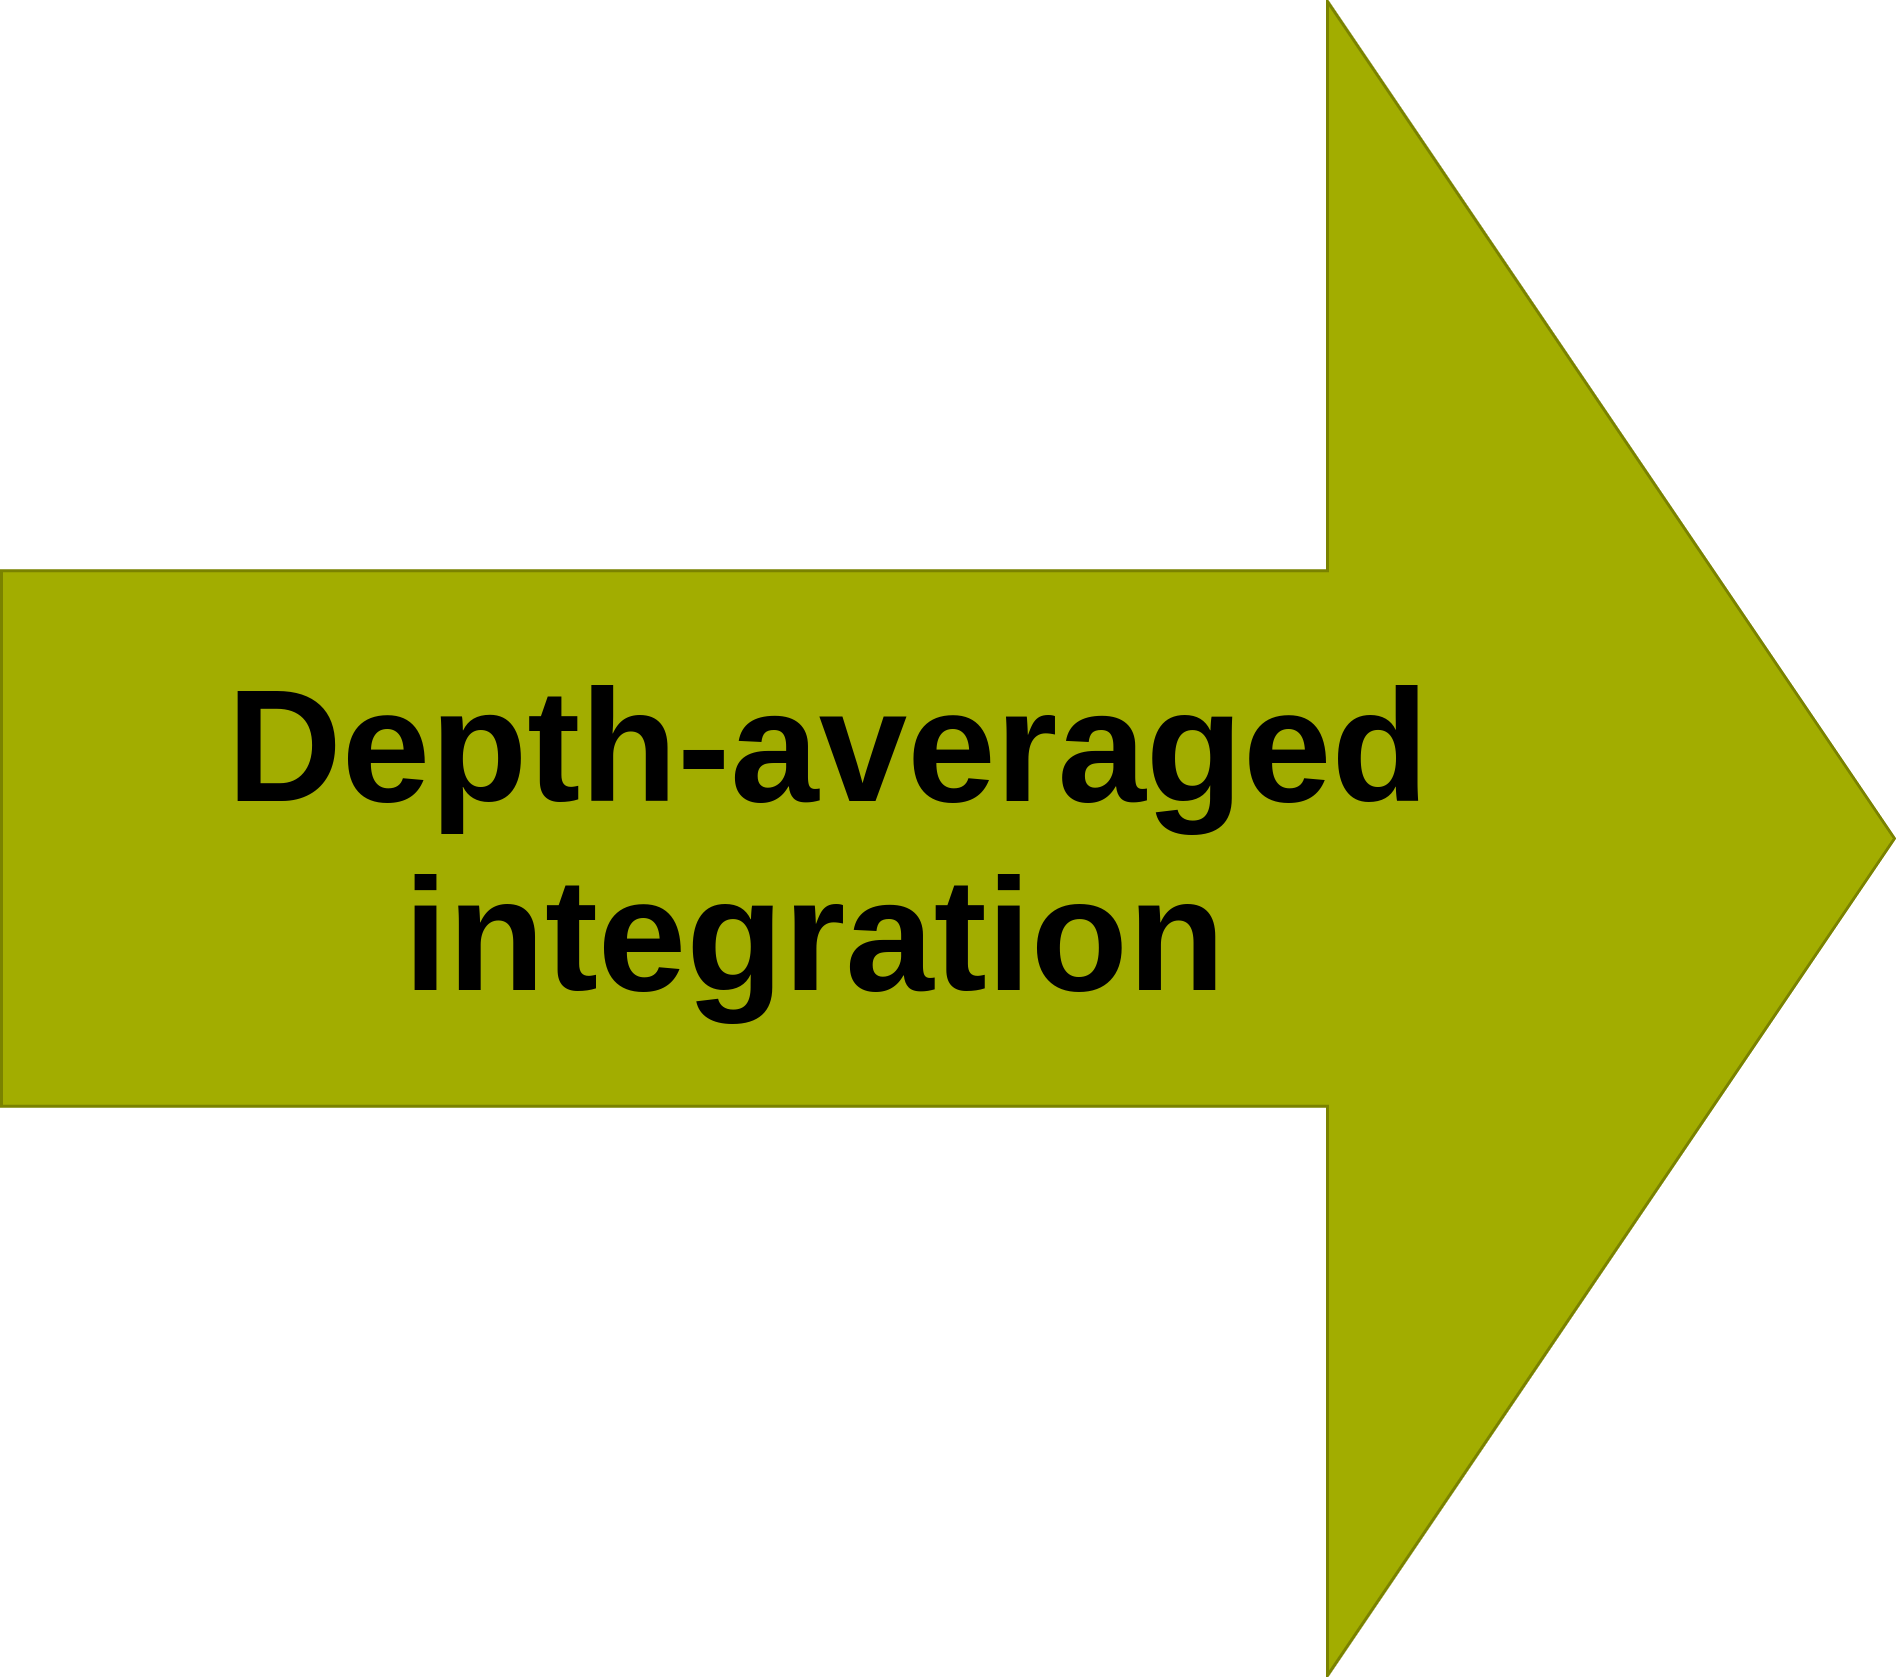
\includegraphics[width=1\textwidth]{Resources/Images/arrow3.png}\\
%\item<3->[] {\LARGE  \makebox[\textwidth]{+}}
%\item<3->[] {\Large \makebox[\textwidth]{\myTUMgreen{Depth-Averaged}}}
%\item<3->[] {\Large \makebox[\textwidth]{\myTUMgreen{Integration}}}
\end{itemize}           
\end{minipage}
\hspace{1cm}
\begin{minipage}{0.4\textwidth}
\begin{itemize}
\item<3->[]
\begin{tcolorbox}[title=SWE model, colback=white] 
\begin{align*}
\myTUMgreen{\frac{\partial h}{\partial t}} + \frac{\partial \myTUMgreen{h}u}{\partial x} + \frac{\partial \myTUMgreen{h}v}{\partial y} &= 0\\[0.5cm]
\frac{\partial \myTUMgreen{hu}}{\partial t} + \frac{\partial}{\partial x}(\myTUMgreen{hu^2} + \myTUMdarkblue{\frac{1}{2} g h^2}) + \frac{\partial \myTUMgreen{huv}}{\partial y} &= \myTUMdarkblue{- gh\frac{\partial b}{\partial x}} \\[0.5cm]
\frac{\partial \myTUMgreen{hv}}{\partial t} + \frac{\partial \myTUMgreen{huv}}{\partial x} + \frac{\partial}{\partial y}(\myTUMgreen{hv^2} + \myTUMdarkblue{\frac{1}{2} g h^2})&= \myTUMdarkblue{- gh\frac{\partial b}{\partial y} }
\end{align*}
\end{tcolorbox}
\end{itemize}
\end{minipage}
\end{frame}
\clearpage


%%%%%%%%%%%%%%%%%%%%
%%%%%%%%%%%%%%%%%%%%
\begin{frame}
    \shiftedframetitle{2. Theory -  \large Shallow Water Equations  model {\small(cont)}}
%\vspace{-2mm}
%\begin{columns}
\begin{minipage}{0.35\textwidth}
\begin{itemize}
\item<1->[] SWE model can be represented as a {\color{TUMBlauDunkel}matrix} form \dots
% derived from mass and momentum conservation laws, and depth averaging \dots %also derived by vertical averaging from the 3d incompressible ns eqs
\item<1->[]
\begin{align*}
\vspace{-15pt}
&\begin{bmatrix}[1.3]
\myTUMdarkblue{h}\\
\myTUMdarkblue{hu}\\
\myTUMdarkblue{hv}\\
\end{bmatrix}_t \ + \
\begin{bmatrix}[1.0]
hu\\
hu^2 + \frac{1}{2}gh^2\\
huv\\
\end{bmatrix}_x\ + \
\begin{bmatrix}[1.0]
hv\\
huv\\
hv^2 + \frac{1}{2}gh^2\\
\end{bmatrix}_y =
\begin{bmatrix}[1.0]
0\\
-gh\ b_x\\
-gh\ b_y
\end{bmatrix}\\[2em]
%&\bar{q} = \begin{bmatrix}[1.3]
%\myTUMdarkblue{h}\\
%\myTUMdarkblue{hu}\\
%\myTUMdarkblue{hv}
%\end{bmatrix}
%\begin{matrix}[1.0]
%\text{\hspace{-3em}\myTUMdarkblue{$\rightarrow\ $\textit{height}}}\\
%\text{\hspace{-2pt}\myTUMdarkblue{$\rightarrow\ $\textit{discharge in x}}} \\
%\text{\hspace{5pt}\myTUMdarkblue{$\rightarrow\ $\textit{discharge in y}}}
%\end{matrix}
&\qquad \lambda^x = 
\begin{bmatrix}[1.0]
u - c\\
u\\
u+c
\end{bmatrix}
,\qquad  \lambda^y = 
\begin{bmatrix}[1.0]
v - c\\
v\\
v+c
\end{bmatrix}
,\qquad c = \sqrt{gh}
\end{align*}
\item<2->[]
\begin{align*}
\qquad \qquad \frac{\partial \myTUMdarkblue{\bar{q}}}{\partial t} + \dfrac{\partial F(\myTUMdarkblue{\bar{q}})}{\partial x} + &\frac{\partial G(\myTUMdarkblue{\bar{q}})}{\partial y} = S(h,x,y,t)
\end{align*}
\end{itemize}
\end{minipage}
\begin{minipage}{0.45\textwidth}  
\begin{itemize}[leftmargin=*]
\item<1->[]
\vspace{2cm}
\begin{center}
\begin{figure}
\includegraphics[scale=0.55]{./Resources/Images/imagesThesis/floor.png}%
\caption{SWE variables schematic}
\label{fig:swechemedit}
\end{figure}
\end{center}
\end{itemize}
\end{minipage}
%\end{columns}

\end{frame}
\clearpage


%%%%%%%%%%%%%%%%%%%%
%%%%%%%%%%%%%%%%%%%
\begin{frame}
    \shiftedframetitle{2. Theory - \large Shallow Water Equations  model {\small(final)}}
\begin{itemize}
\setlength\itemsep{1.8em}
\item<1-> \textbf{simplify} \textit{$3D$} Navier-Stokes \textit{to} a \textit{$2D$} system of equations
\item<1-> \textit{\textbf{neglect} vertical velocity}:  $ W \ll U,V $, horizontal distances $L$ $\gg$ vertical distance $H$
\item<1-> represent a \textbf{hyperbolic PDE} system $\rightarrow$ Riemann Problem and FVM
\item<1-> \textbf{Applications}: 
\begin{itemize}
\addtolength{\itemindent}{1cm}
\item \textit{Free surface flows} around structures, 
\item \textit{tsunamis} prediction,
\item \textit{atmospheric flows}, \dots
\end{itemize}
%\end{itemize}
%\end{tcolorbox}
%\addtolength{\leftmargini}{-0.8cm}
%\begin{itemize}
\item<2->[]
\begin{tcolorbox}[%colframe=TUMGreen,
colback=white] 
\textbf{Both NS and SWE reach a solution for free-surface problems $\rightarrow$ compatibility between the respective solution methods}
\end{tcolorbox}
\end{itemize}
%\end{minipage}
\end{frame}
\clearpage

%%%%%%%%%%%%%%%

\begin{frame}
    \shiftedframetitle{2. Theory - \large Flow characterization}
    \hspace{0.8cm}
\begin{minipage}{0.45\textwidth}
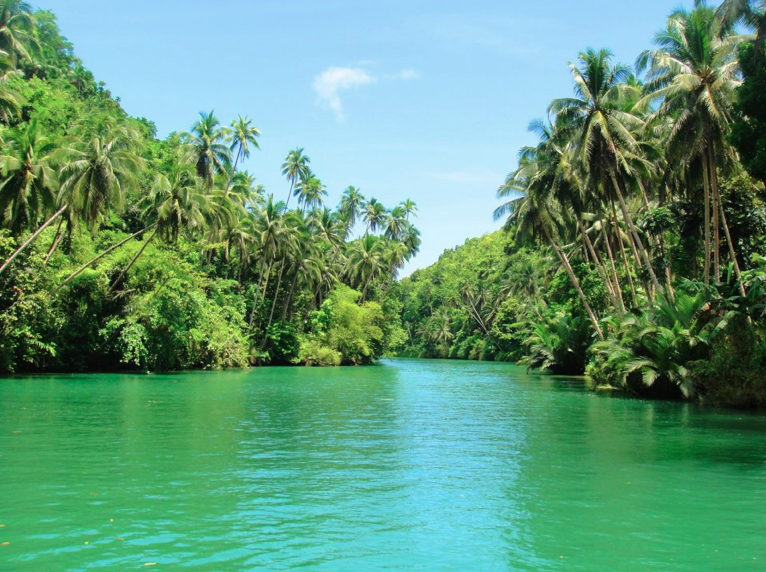
\includegraphics[width=1\textwidth]{Resources/Images/calmriver.png}
\end{minipage}
\hspace{1.1cm}
\begin{minipage}{0.45\textwidth}
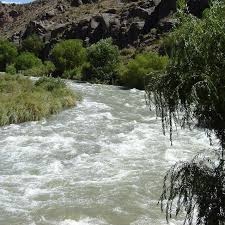
\includegraphics[width=0.75\textwidth]{Resources/Images/fastriver.jpeg}
\end{minipage}
\end{frame}

%%%%%%%%%%%%%%%%%
%%%%%%%%%%%%%%%%%
\begin{frame}
    \shiftedframetitle{2. Theory - \large Flow characterization}
\begin{minipage}{0.45\textwidth}
\begin{itemize}
\item<1->[] 
\centering
\vspace{-1cm}
\myTUMdarkblue{Subcritical flow}\\[0.5cm]
\hspace{0.2cm}
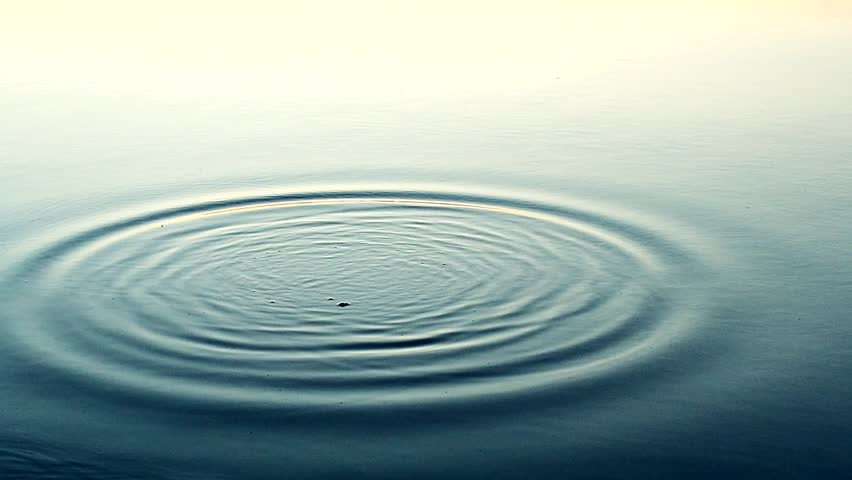
\includegraphics[width=0.6\textwidth]{Resources/Images/waves.jpg}
\\[0.5cm]
\hspace{1.8cm}
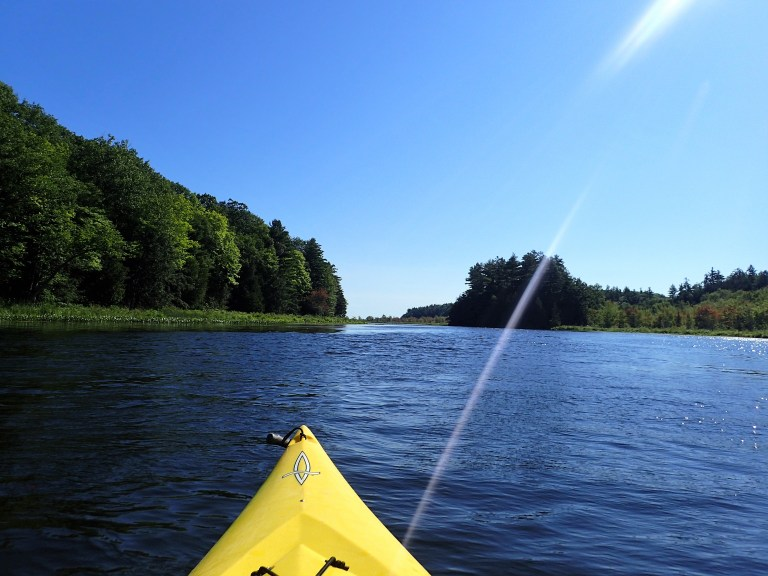
\includegraphics[width=0.6\textwidth]{Resources/Images/paddle.jpg}
\end{itemize}
\end{minipage}
%\hspace{1cm}
\begin{minipage}{0.45\textwidth}
\begin{itemize}
\item<2->[]
\centering
\myTUMdarkblue{Supercritical flow}\\[0.5cm]
\hspace{0.25cm}
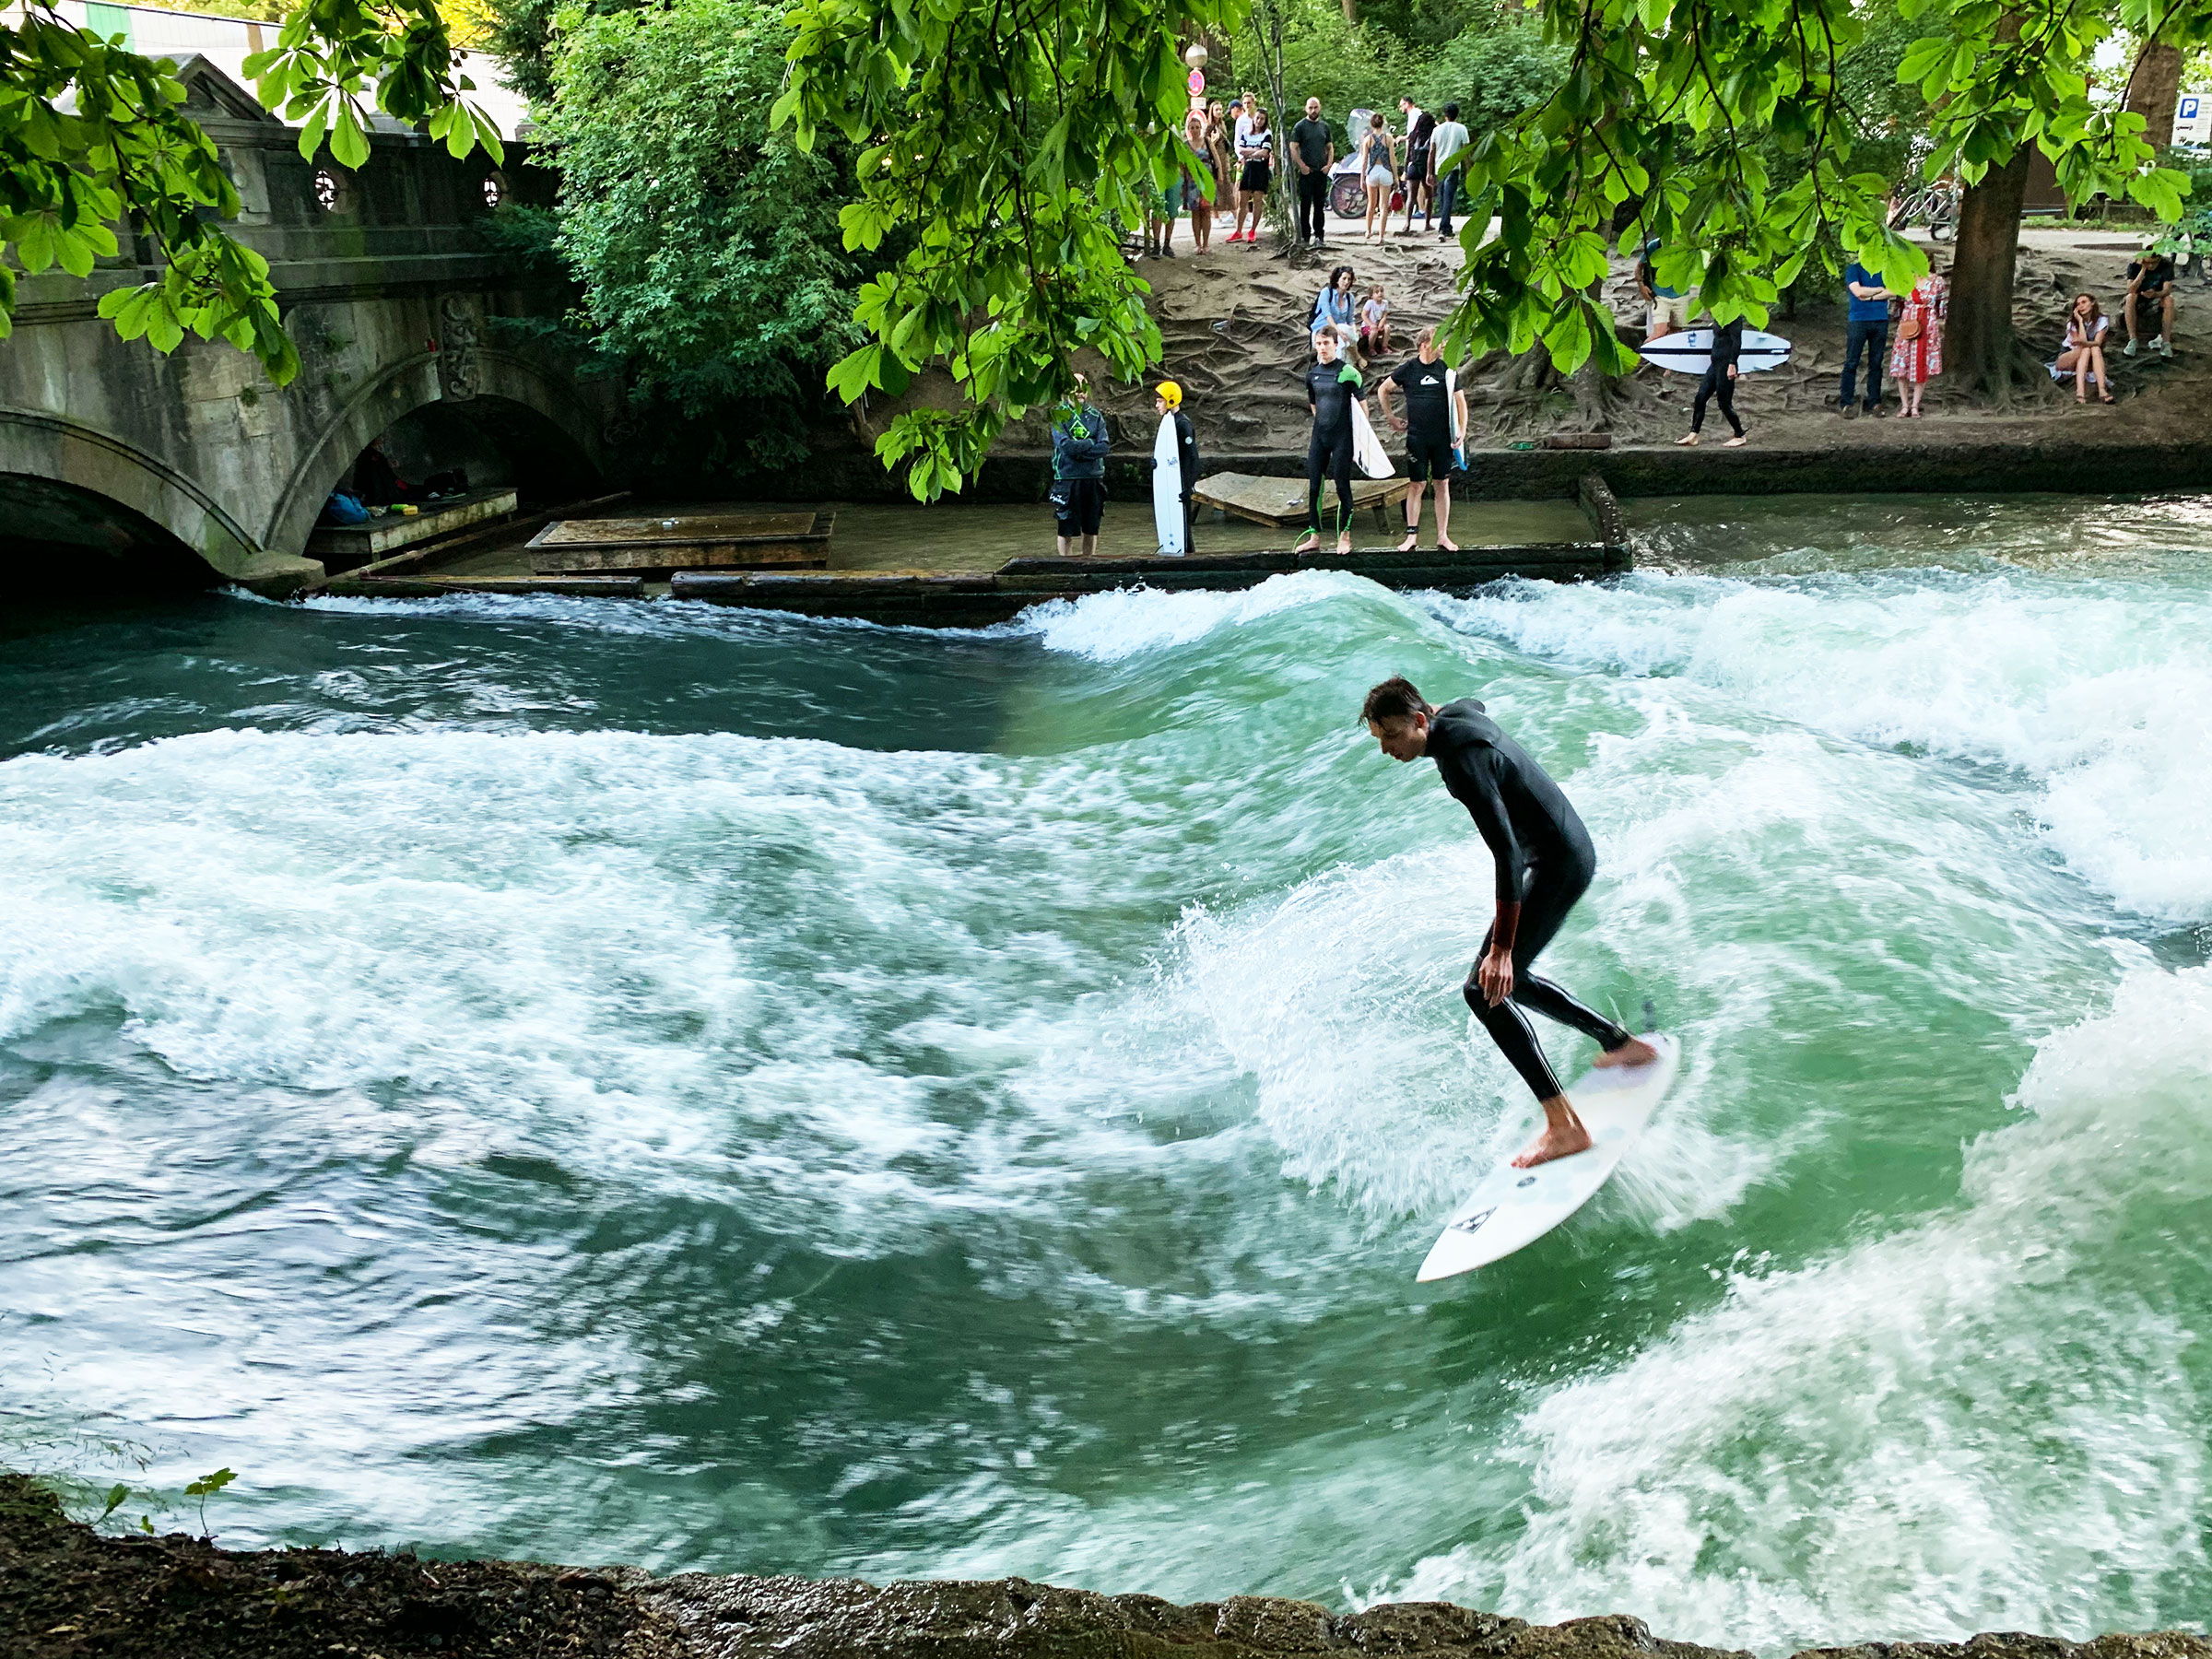
\includegraphics[width=0.8\textwidth]{Resources/Images/eisbach.jpg}\\[0.5cm]
\hspace{2cm}
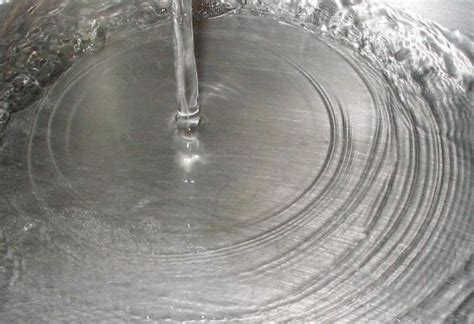
\includegraphics[width=0.5\textwidth]{Resources/Images/faucet.jpeg} 
\end{itemize}
\end{minipage}
\end{frame}

\clearpage



%%%%%%%%%%%%%%%%%
%%%%%%%%%%%%%%%%%
\begin{frame}
    \shiftedframetitle{2. Theory - \large Flow characterization}
\begin{minipage}{0.45\textwidth}
\begin{itemize}
\item<1->[] 
\centering
\myTUMdarkblue{Subcritical flow}\\[0.5cm]
\hspace{0.2cm}
\begin{minipage}{0.4\textwidth}
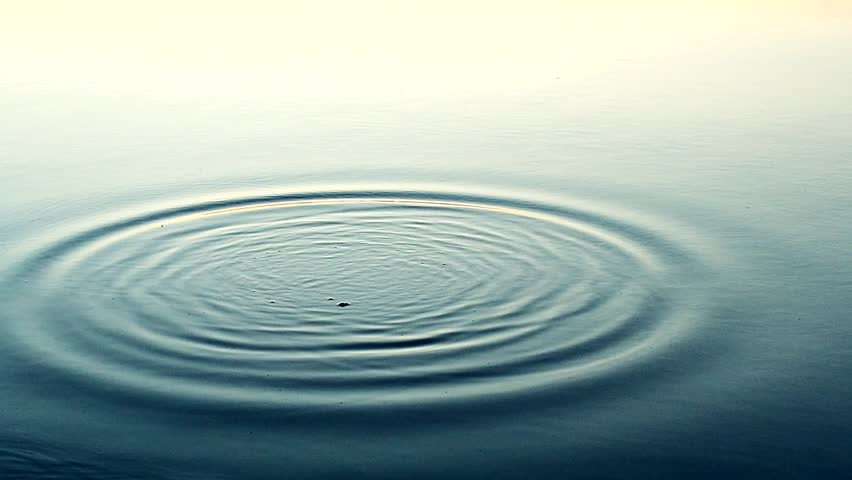
\includegraphics[width=1\textwidth]{Resources/Images/waves.jpg}
\end{minipage}
\begin{minipage}{0.45\textwidth}
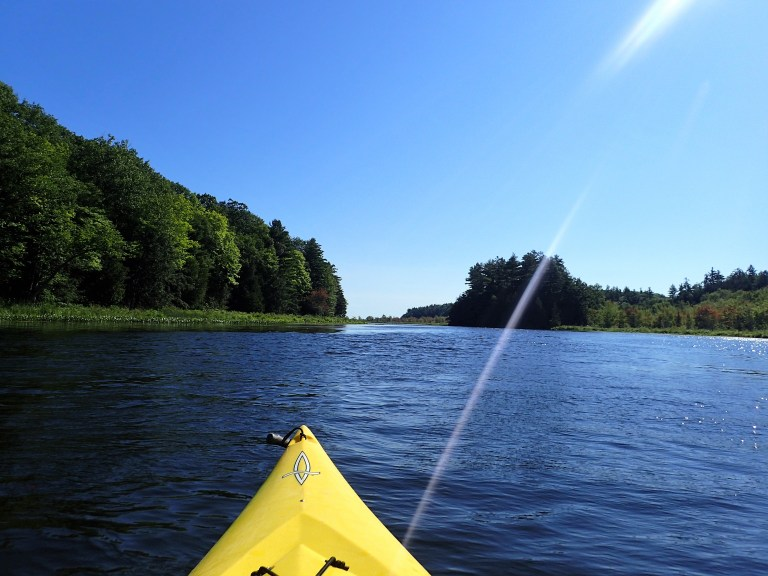
\includegraphics[width=0.67\textwidth]{Resources/Images/paddle.jpg}
\end{minipage}\\[0.5cm]
\hspace{0.25cm}
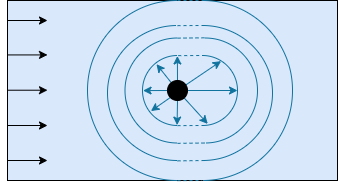
\includegraphics[width=0.75\textwidth]{Resources/Images/subcritical.png}
\end{itemize}
\end{minipage}
%\hspace{1cm}
\begin{minipage}{0.4\textwidth}
\centering
\begin{itemize}
\item<2->[]
\centering
\myTUMdarkblue{Supercritical flow}\\[0.5cm]
\hspace{0.25cm}
\begin{minipage}{0.4\textwidth}
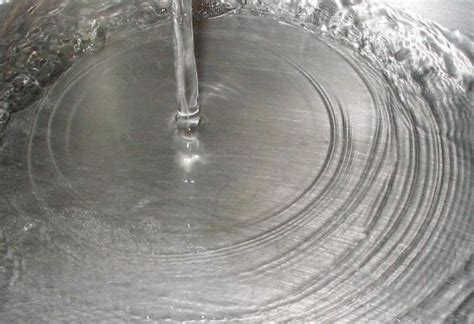
\includegraphics[width=0.98\textwidth]{Resources/Images/faucet.jpeg}
\end{minipage}
\begin{minipage}{0.45\textwidth}
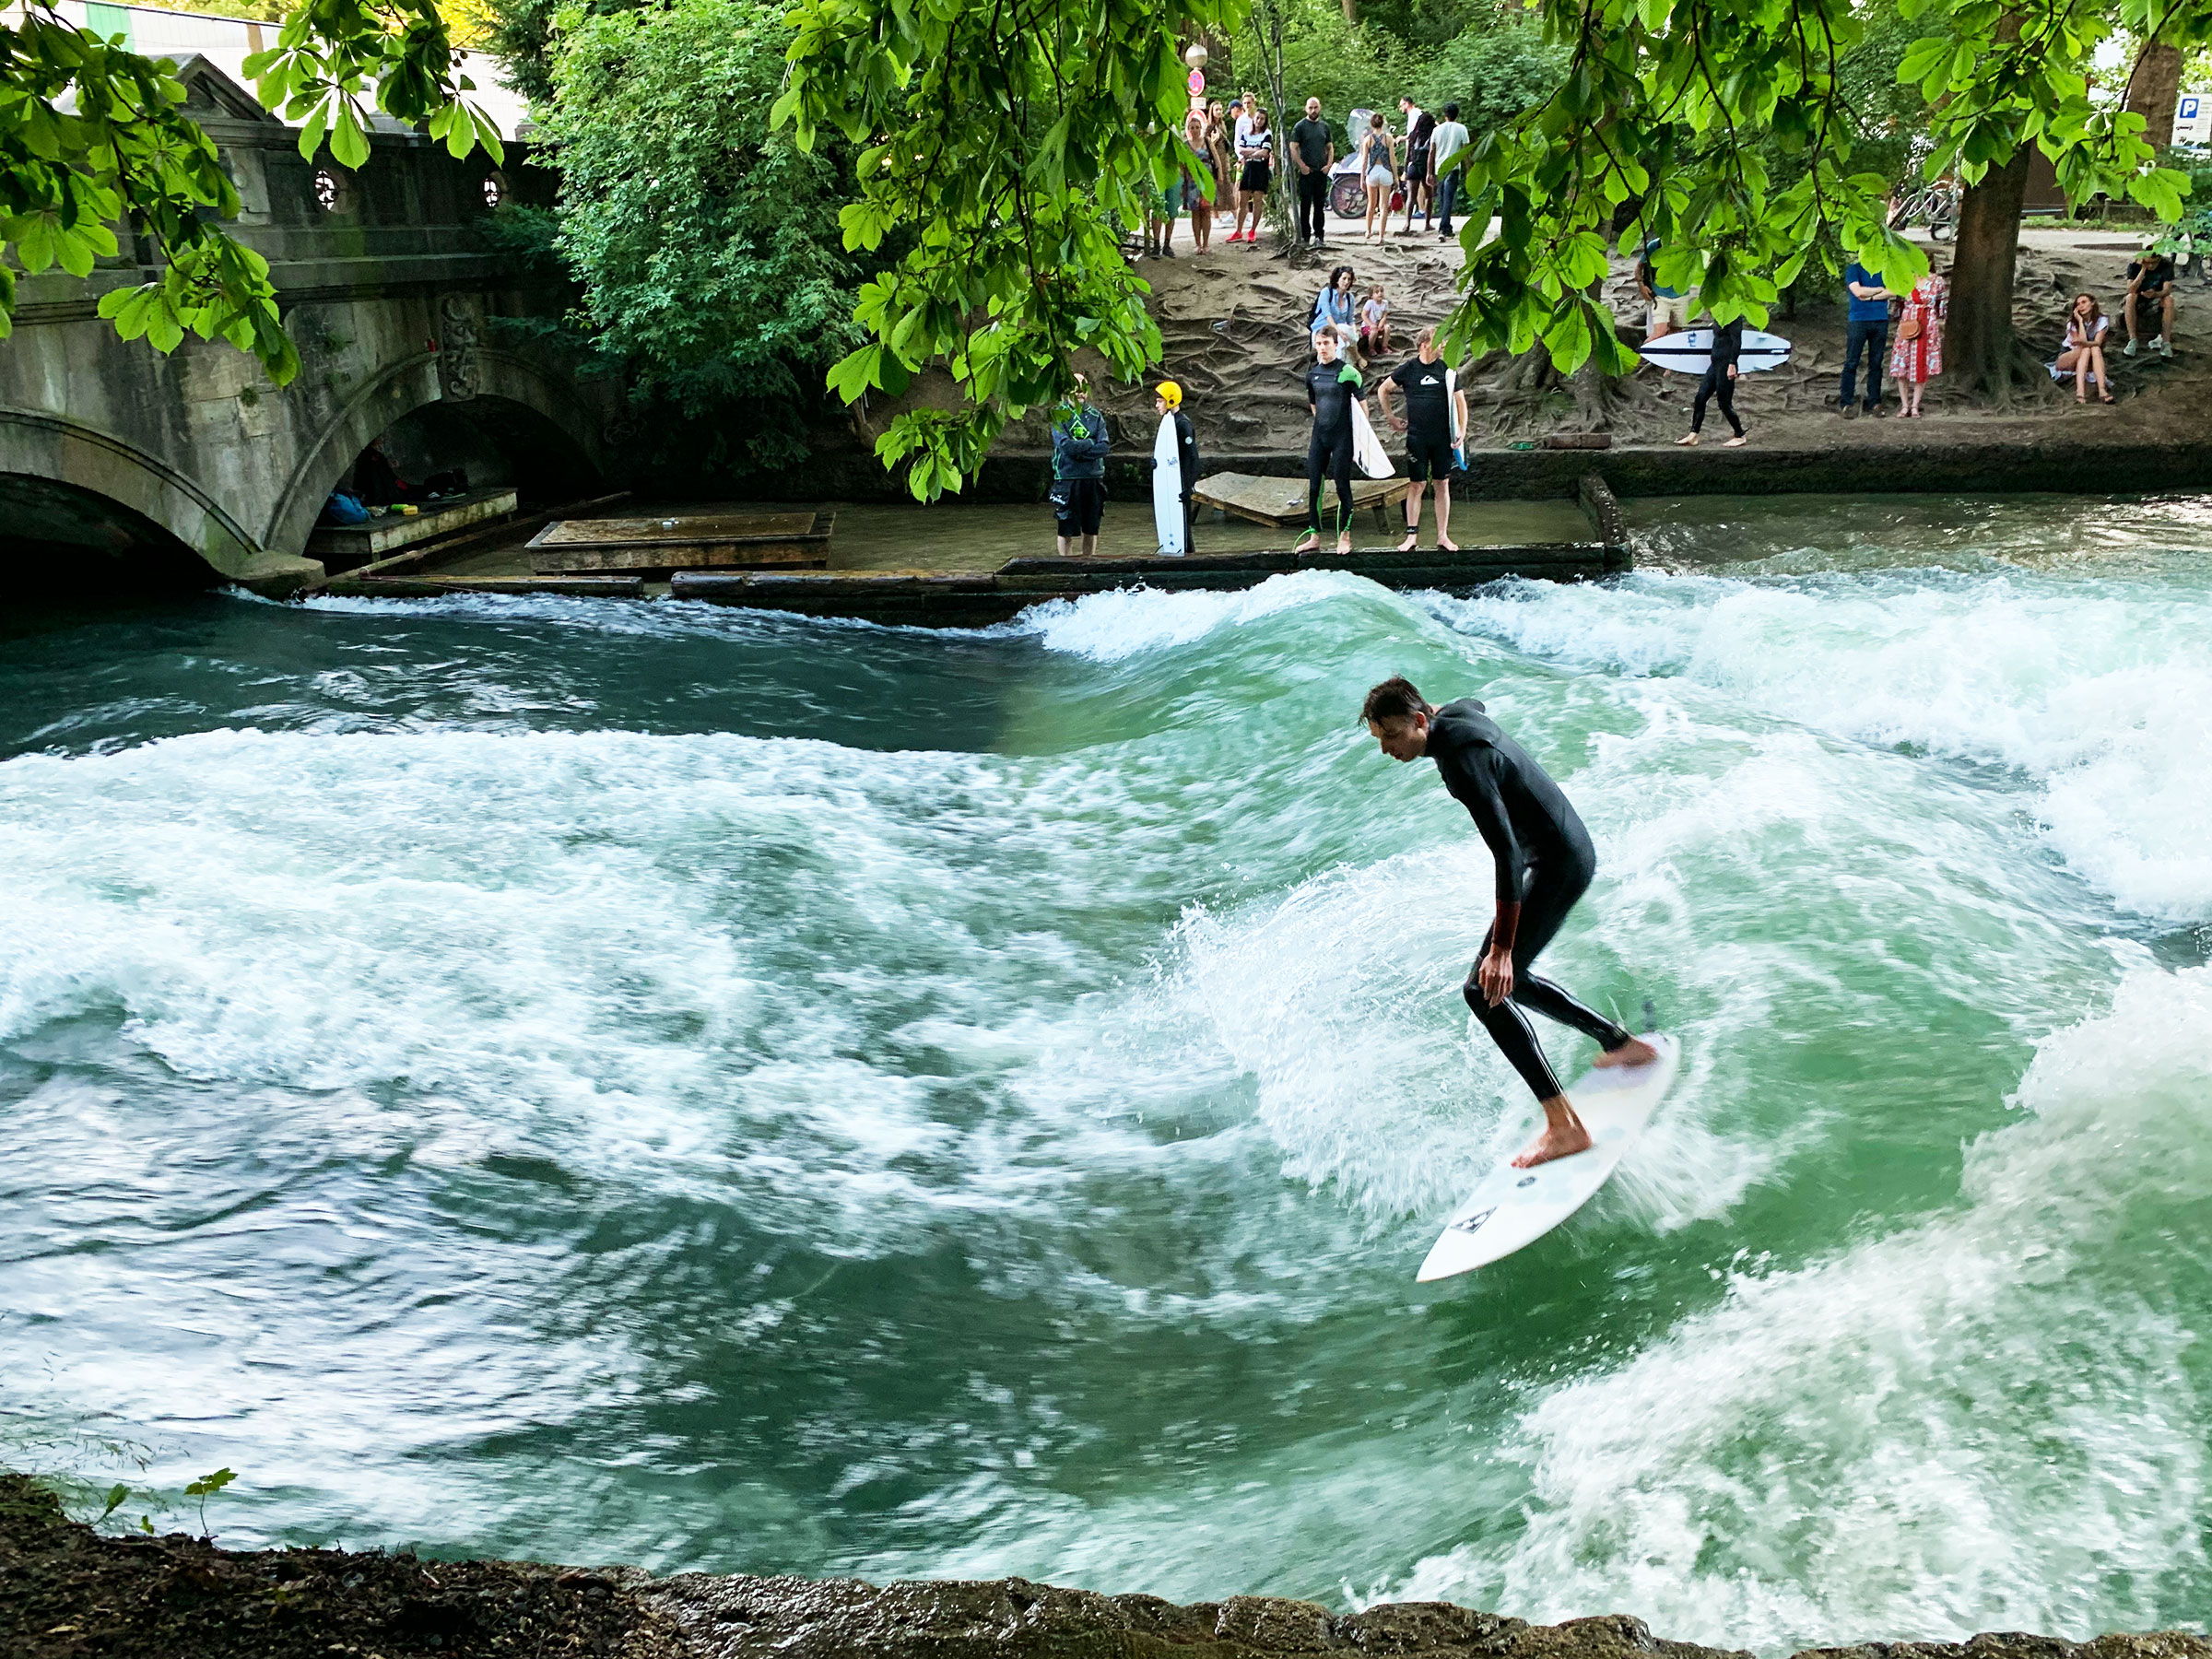
\includegraphics[width=0.78\textwidth]{Resources/Images/eisbach.jpg}
\end{minipage}\\[0.4cm]
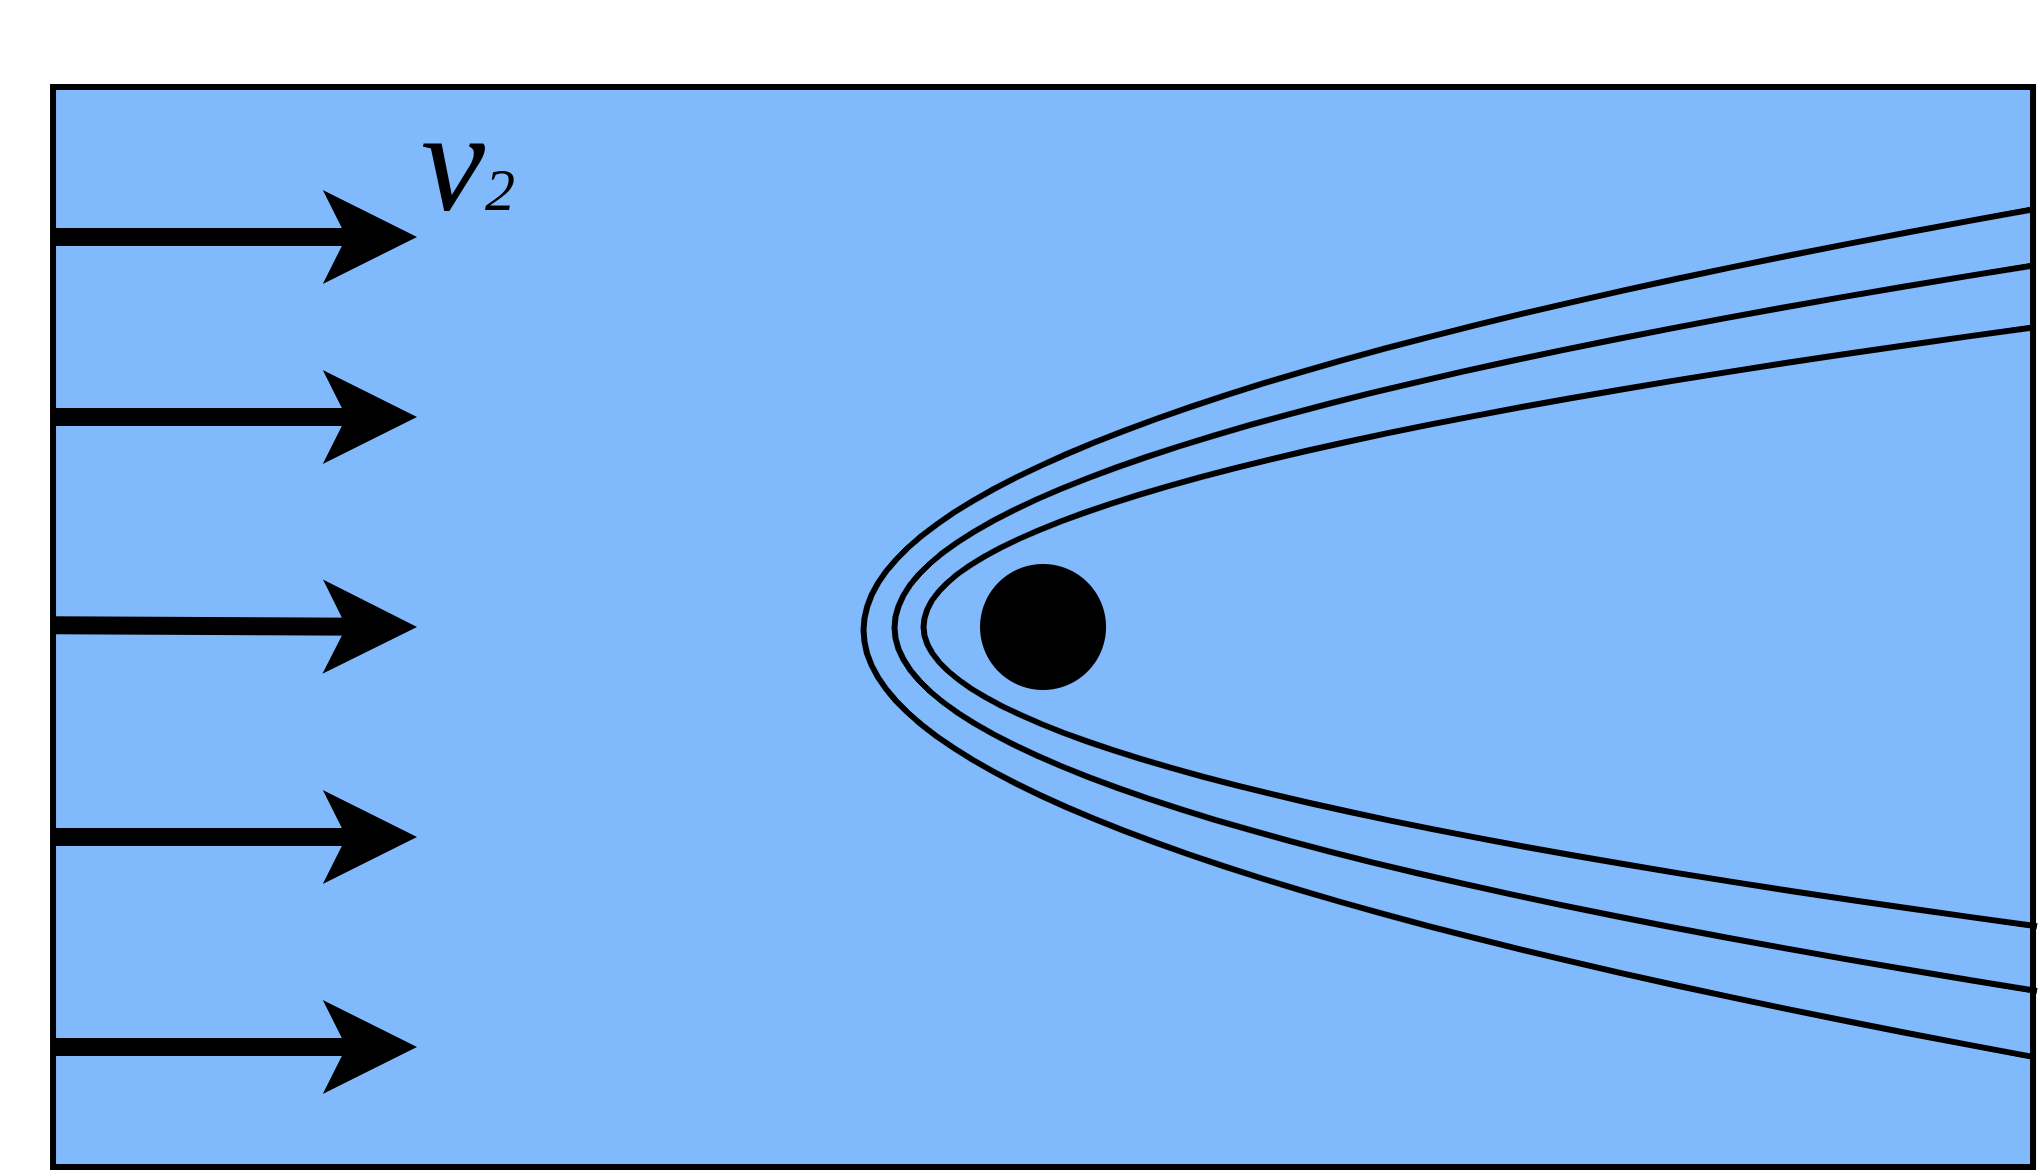
\includegraphics[width=0.85\textwidth]{Resources/Images/supercritical.png}
\end{itemize}
\end{minipage}
\end{frame}

\clearpage


%%%%%%%%%%%%%%%%
%%%%%%%%%%%%%%%%
\begin{frame}
    \shiftedframetitle{2. Theory - \large Flow characterization \small(cont)}
\begin{minipage}{0.5\textwidth}
\vspace{1cm}
\includegraphics[width=\textwidth]{Resources/Images/imagesThesis/hydjump.png}
\end{minipage}
\hspace{1cm}
\begin{minipage}{0.4\textwidth}
\vspace{1.5cm}
\begin{tcolorbox}[colback=white] 
\begin{itemize}
\setlength{\itemsep}{1cm}
\item[] $\mathbf{Fr = \dfrac{v}{c} =\dfrac{V}{\sqrt{gh}} \propto \dfrac{inertia\ force}{gravity\ force}}$
\item Supercritical $\sqrt{gh}\ < V$
\item Subcritical $\sqrt{gh}\ > V$
\item Critical $\sqrt{gh}\  =  V$
\end{itemize}
\end{tcolorbox}
\end{minipage}
\end{frame}
